% Title page.
\title[Aula 04]{Oceanografia Física Descritiva}
\subtitle{Revisão de Matemática e Física}
\author[Filipe Fernandes]{Filipe P. A. Fernandes}
\institute[unimonte]{Centro Universitário Monte Serrat}
\date[Setembro 2013]{12 de Setembro 2013}

\logo{
\includegraphics[scale=0.15]{../common/university_logo.png}}

\begin{document}

% The title page frame.
\begin{frame}[plain]
  \titlepage
\end{frame}

\section*{Outline}
\begin{frame}
\tableofcontents
\end{frame}

\section{Revisão}
\section{Sistema de coordenadas}

\begin{frame}
\frametitle{Sistema de coordenadas}
  \begin{block}{}
    Sistema de coordenadas da ``mão direita''.
  \end{block}

  \vspace{0.3cm}

  \begin{columns}
    \begin{column}{0.5\textwidth}
      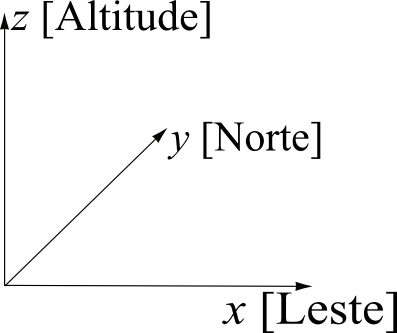
\includegraphics[scale=0.4]{./figures/coordinates_space.png}
    \end{column}

    \begin{column}{0.5\textwidth}
      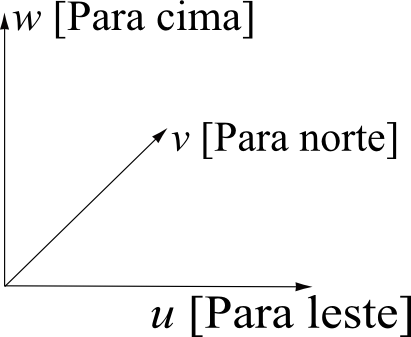
\includegraphics[scale=0.4]{./figures/coordinates_velocity.png}
    \end{column}
  \end{columns}

  \vspace{0.5cm} \pause

  \scriptsize{obs: As correntes oceânica são nomeadas para a direção que
              viajam.  Isto é o oposto do usado em meteorologia!}
\end{frame}


\section{Vetores}

\subsection{Notações}
\begin{frame}
\frametitle{Notação de Vetores}

  \begin{itemize}[<+-| alert@+>]
    \item Escalar $a$ ou $|\vec{a}|$:

    \begin{enumerate}[<+-| alert@+>]
      \item Apenas magnitude;
      \item Exemplos: Temperatura, Salinidade, Pressão, etc.
    \end{enumerate}

    \item Vetores $\vec{a}$ ou $\mathbf{a}$:

    \begin{enumerate}[<+-| alert@+>]
      \item Magnitude e Direção;
      \item Exemplos: Deslocamento = distância (escalar) ``mais'' direção.
    \end{enumerate}
  \end{itemize}
  \pause
    \begin{center}
      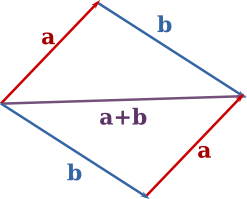
\includegraphics[scale=0.4]{./figures/vector_addition.png}
    \end{center}
\end{frame}


\subsection{Produto vetorial e escalar}

\begin{frame}
\frametitle{Vetores em componentes escalares}
  \begin{block}{}
    Resolvendo vetores em componentes escalares para um sistema de coordenadas
    2D.
  \end{block}

  \begin{columns}
    \begin{column}{0.5\textwidth}
      \begin{center}
        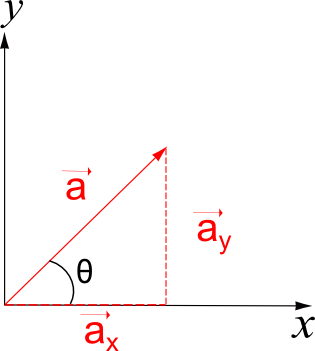
\includegraphics[scale=0.5]{./figures/vector2scalar.png}
      \end{center}
    \end{column}

    \begin{column}{0.5\textwidth}
      \begin{itemize}
        \item $a_x = |\vec{a}|\cos(\theta)$
        \item $a_y = |\vec{a}|\sin(\theta)$
      \end{itemize}
    \end{column}
  \end{columns}

\end{frame}


\begin{frame}
\frametitle{Operações com vetores}
  \begin{itemize}[<+-| alert@+>]
    \item Produto escalar:
      \begin{enumerate}[<+-| alert@+>]
        \item Dois vetores produzem um escalar;
        \item $|\vec{a}| \cdot |\vec{b}| = |\vec{a}||\vec{b}|\cos(\theta)$
      \end{enumerate}
    \item Produto vetorial:
      \begin{enumerate}[<+-| alert@+>]
        \item Dois vetores produzem um novo vetor ortogonal aos mesmos;
        \item $|\vec{a}| \times |\vec{b}| = |\vec{a}||\vec{b}|\sin(\theta)$
      \end{enumerate}
  \end{itemize}
\end{frame}

\section{Derivadas}

\begin{frame}
\frametitle{Derivadas}

  \begin{itemize}[<+-| alert@+>]
    \item Derivada = a taxa instantânea de mudança de uma função;
    \item Ou a reta tangente a função;
    \item $\frac{dy}{dx}$ é a mudança de $y$ com respeito a $x$, onde
          $y = f(x)$.
    \item Também escrito na forma de $f'(x)$.
  \end{itemize}

\end{frame}


\begin{frame}
\frametitle{Derivadas}

  \begin{itemize}[<+-| alert@+>]
    \item $f(x) = x^4 + \sin(x^2) - \ln(x)e^x + 7$
    \item $f'(x) = 4x^{(4-1)} + \frac{d(x^2)}{dx}\cos(x^2) -
          \frac{d(\ln x)}{dx}e^x - \ln x\frac{d(e^x)}{dx}+ 0$
    \item $= 4x^3 + 2x\cos(x^2) - \frac{1}{x}e^x - \ln(x)e^x$
  \end{itemize}

  \pause Lembram?

\end{frame}


\begin{frame}
\frametitle{Derivadas}

  \begin{itemize}[<+-| alert@+>]
    \item Regra da potência:
      \begin{enumerate}[<+-| alert@+>]
        \item $f(x) = x^a$, para qualquer numero real $a$;
        \item $f'(x) = ax^{(a-1)}$
      \end{enumerate}
    \item Regra da cadeia:
      \begin{enumerate}[<+-| alert@+>]
        \item $f(x) = h(g(x))$, logo
        \item $f'(x) = h'(g(x)) \times g'(x)$
      \end{enumerate}
    \item Regra do produto:
      \begin{enumerate}[<+-| alert@+>]
        \item $(fg)' = f'g + fg'$
      \end{enumerate}
    \item Regra da constante:
      \begin{enumerate}[<+-| alert@+>]
        \item A derivada de qualquer constante é zero.
        \item Para $c f(x)$, a derivada é $c f'(x)$.
      \end{enumerate}
  \end{itemize}

\end{frame}


\subsection{Derivadas parciais}

\begin{frame}
\frametitle{Derivadas parciais}

  \begin{itemize}[<+-| alert@+>]
    \item Derivadas parciais -- a derivada tomada com respeito com apenas uma
          variável de uma função, enquanto mantemos as outras variáveis
          constantes.
    \item $\frac{\partial f}{\partial x}$ ou $f_x$
  \end{itemize}

\end{frame}


\begin{frame}
\frametitle{Derivadas parciais}

  \begin{itemize}[<+-| alert@+>]
    \item Exemplo:
      \begin{enumerate}[<+-| alert@+>]
        \item Volume de um cone: $V = \frac{r^2h\pi}{3}$
        \item $r \equiv$ raio
        \item $h \equiv$ altura
        \item Parcial com respeito ao raio:
              $\frac{\partial V}{\partial r} = \frac{2rh\pi}{3}$
        \item Parcial com respeito à altura:
              $\frac{\partial V}{\partial h} = \frac{r^2\pi}{3}$
      \end{enumerate}
  \end{itemize}

\end{frame}


\subsection{O operador ``del'' ($\partial$)}

\begin{frame}
\frametitle{O operador ``del''}

  \begin{itemize}[<+-| alert@+>]
    \item $\nabla$ em 3D:
      \begin{enumerate}[<+-| alert@+>]
        \item $\nabla = \left( \pd{}{x}, \pd{}{y}, \pd{}{z} \right)$
        \item $\nabla = \mathbf{i}\pd{}{x} + \mathbf{j}\pd{}{y} + \mathbf{k}\pd{}{z}$
        \item Note que {\bf i, j, k} estão em negrito, indicando vetores.
              Esses são considerados vetores ``unidade'' com magnitude 1 nas
              direções $x, y, z$ respectivamente.
      \end{enumerate}
      \pause
      $\vec{a} = a_x\mathbf{i} + a_y\vec{j} + a_z{\hat{k}}$
  \end{itemize}

\end{frame}



\subsection{Gradiente, divergente e rotacional}
\begin{frame}
\frametitle{Gradiente}

  \begin{columns}
    \begin{column}{0.5\textwidth}
        \begin{itemize}[<+-| alert@+>]
          \item Representa a direção do crescimento mais rápido da função
                escalar.
            \begin{enumerate}[<+-| alert@+>]
              \item O gradiente de um escalar é um vetor;
              \item $\nabla$ aplicado a uma função $S$:
                    $\vec{\nabla S} = \left(\pd{S}{x}, \pd{S}{y}, \pd{S}{z}
                    \right)$
            \end{enumerate}
        \end{itemize}
    \end{column}
  \pause
    \begin{column}{0.5\textwidth}
      \begin{center}
        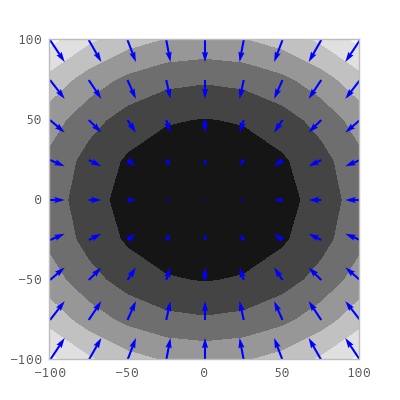
\includegraphics[scale=0.55]{./figures/gradient.png}
      \end{center}
    \end{column}
  \end{columns}

\end{frame}


\begin{frame}
\frametitle{Divergente}

  \begin{columns}
    \begin{column}{0.5\textwidth}
        \begin{itemize}[<+-| alert@+>]
          \item Representa a tendência de um campo vetorial de se ``originar''
                de ou de convergir em um certo ponto.
            \begin{enumerate}[<+-| alert@+>]
              \item Produto escalar entre dois vetores resulta um escalar;
              \item $\text{div }\mathbf{U} =
                    \nabla \cdot \mathbf{U} =
                    \pd{u}{x} + \pd{v}{y} + \pd{w}{z}$
              \item Onde $\mathbf{U} = u\vec{i}  +  v\vec{j} + w\vec{k}$
            \end{enumerate}
        \end{itemize}
    \end{column}
    \pause
    \begin{column}{0.5\textwidth}
      \begin{center}
        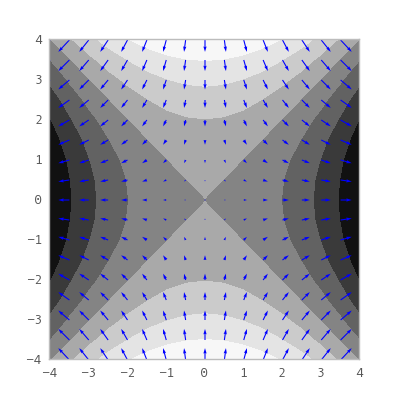
\includegraphics[scale=0.55]{./figures/divergence.png}
      \end{center}
    \end{column}
  \end{columns}

\end{frame}


\begin{frame}
\frametitle{Rotacional}

  \begin{columns}
    \begin{column}{0.5\textwidth}
        \begin{itemize}[<+-| alert@+>]
          \item Representa a tendência de um campo vetorial de ``girar'' sob um
                certo ponto.
            \begin{enumerate}[<+-| alert@+>]
              \item Produto vetorial entre dois vetores resulta um vetor;
              \item $\text{curl } \mathbf{U} = \nabla \times \mathbf{U} = $
            \end{enumerate}
        \end{itemize}  \pause
                \begin{equation*}
                  \begin{bmatrix}
                    \mathbf{i} & \mathbf{j} & \mathbf{k}\\
                    \pd{}{x} & \pd{}{y} & \pd{}{z}\\
                    u & v & w
                  \end{bmatrix} =
                  \begin{bmatrix}
                    \pd{w}{y} - \pd{v}{z}\\
                    \pd{u}{z} - \pd{w}{x}\\
                    \pd{v}{x} - \pd{u}{y}
                  \end{bmatrix}
                \end{equation*}
    \end{column}
    \pause
    \begin{column}{0.5\textwidth}
      \begin{center}
        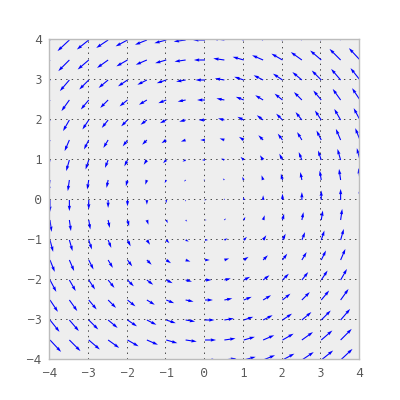
\includegraphics[scale=0.55]{./figures/curl.png}
      \end{center}
    \end{column}
  \end{columns}

\end{frame}

\section{Leis e equações do movimento}

\begin{frame}
\frametitle{Leis de movimento de Newton}

  \begin{itemize}[<+-| alert@+>]
    \item Primeira lei:
      \begin{enumerate}[<+-| alert@+>]
        \item Na ausência de forças externas um corpo permanecerá em velocidade constante ou em repouso (dependendo da referência)
      \end{enumerate}
    \item Segunda lei:
      \begin{enumerate}[<+-| alert@+>]
        \item Quando observado por um referente inercial a força resultante
              em uma partícula é igual a taxa de mudança do seu momento
              $F = \frac{d(mv)}{dt}$.
              \pause (ou massa é igual a força vezes aceleração.)
      \end{enumerate}
    \item Terceira lei:
      \begin{enumerate}[<+-| alert@+>]
        \item Para toda ação há uma reação igual com sentido contrário.
      \end{enumerate}
  \end{itemize}

\end{frame}


\begin{frame}
\frametitle{Equações de movimento}

  \begin{itemize}[<+-| alert@+>]
    \item Velocidade:
      \begin{enumerate}[<+-| alert@+>]
        \item Rapidez do movimento (escalar)
      \end{enumerate}
    \item Velocidade:
      \begin{enumerate}[<+-| alert@+>]
        \item A rapidez mais uma direção (vetor)
      \end{enumerate}
    \item Aceleração:
      \begin{enumerate}[<+-| alert@+>]
        \item A taxa de mudança da velocidade sob o tempo
        \item aceleração média: $\vec{a} = (\vec{v_f} - \vec{v_i})/t$
      \end{enumerate}
    \item Força:
      \begin{enumerate}[<+-| alert@+>]
        \item Massa $\times$ aceleração: $\vec{F} = m\vec{a}$
      \end{enumerate}
  \end{itemize}
\end{frame}

\begin{frame}
\frametitle{Dever de casa}
    \begin{block}{}
        Ler apêndice Pond e Pickard 1--3.
    \end{block}
\end{frame}

\end{document}
